\pagenumbering{arabic}% resets `page` counter to 1
\renewcommand*{\thepage}{B\arabic{page}}
%\pagestyle{empty}
 
\section{Maps}
\subsection*{Nishijin Plaza}
\fbox{Ground Floor (1F)}\\
\noindent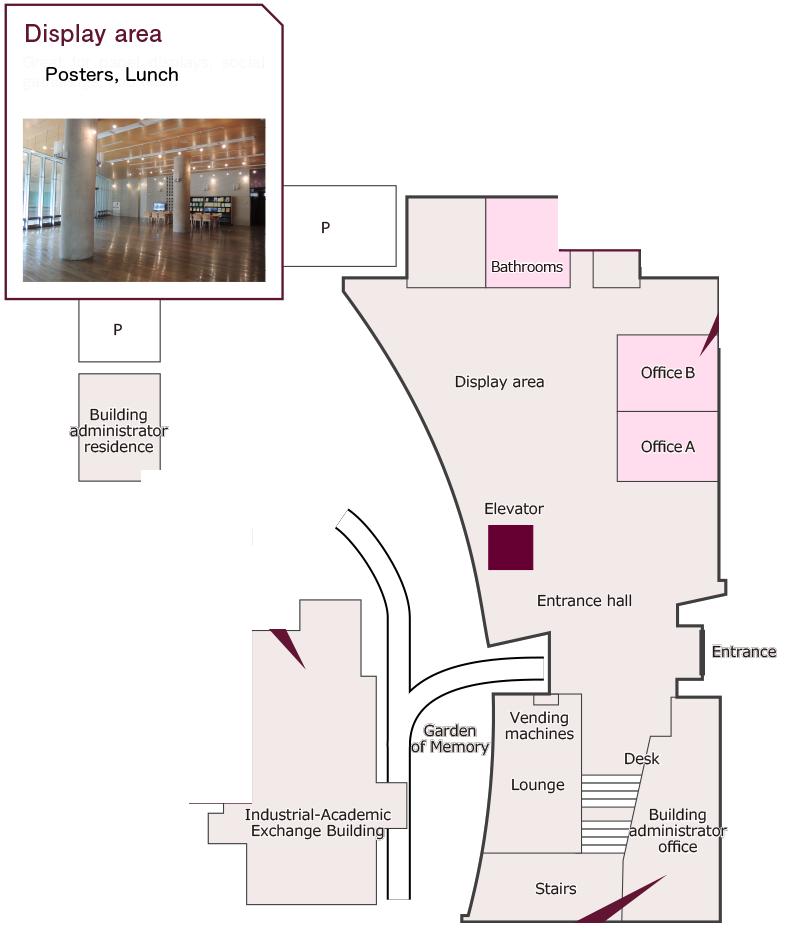
\includegraphics[width=0.95\textwidth]{1F.png}
\newpage
\fbox{First Floor (2F)}\\
\noindent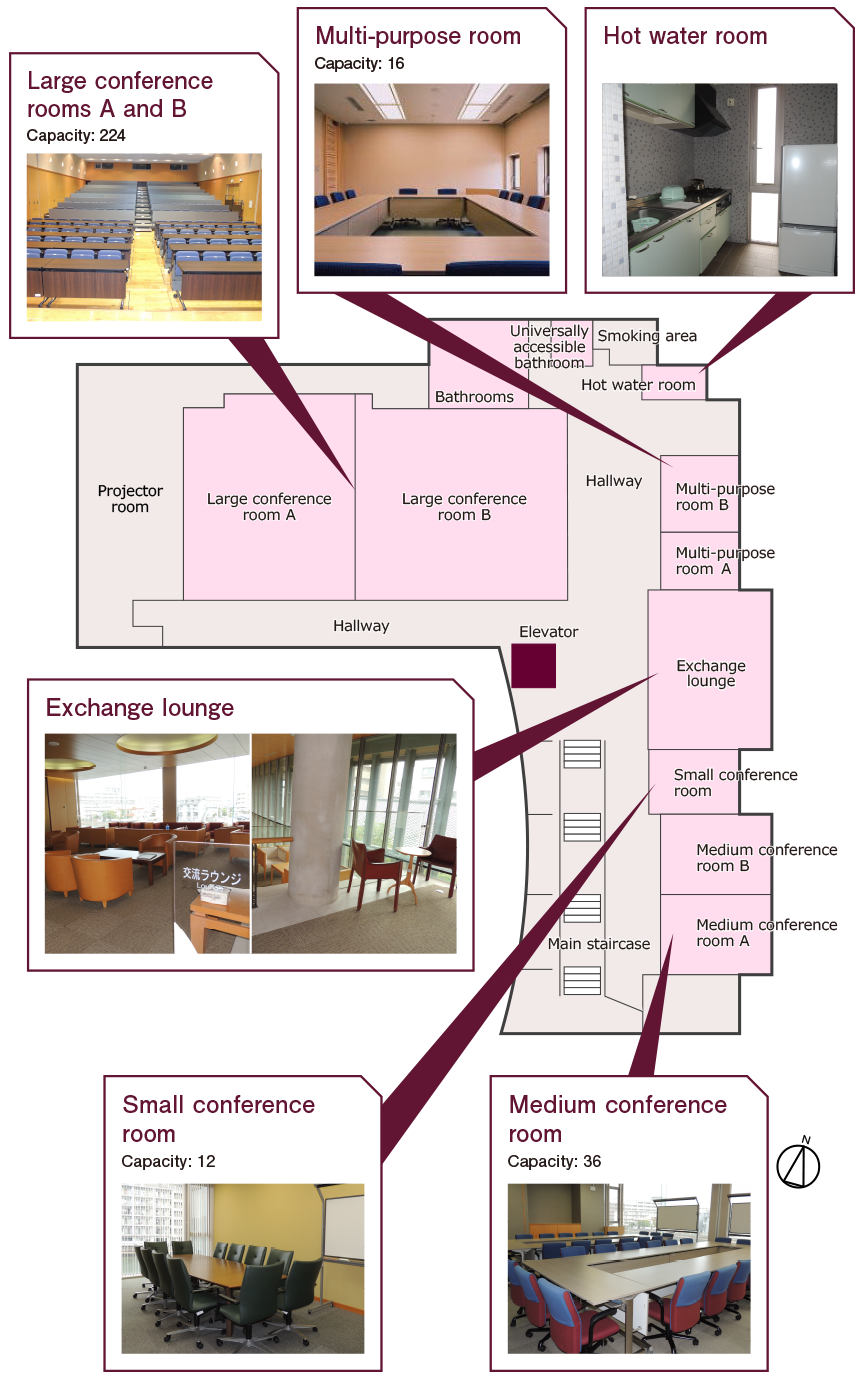
\includegraphics[width=0.832\textwidth]{2F.png}
\newpage

\subsection*{Nishijin Station $\rightarrow$ Nishijin Plaza}
\noindent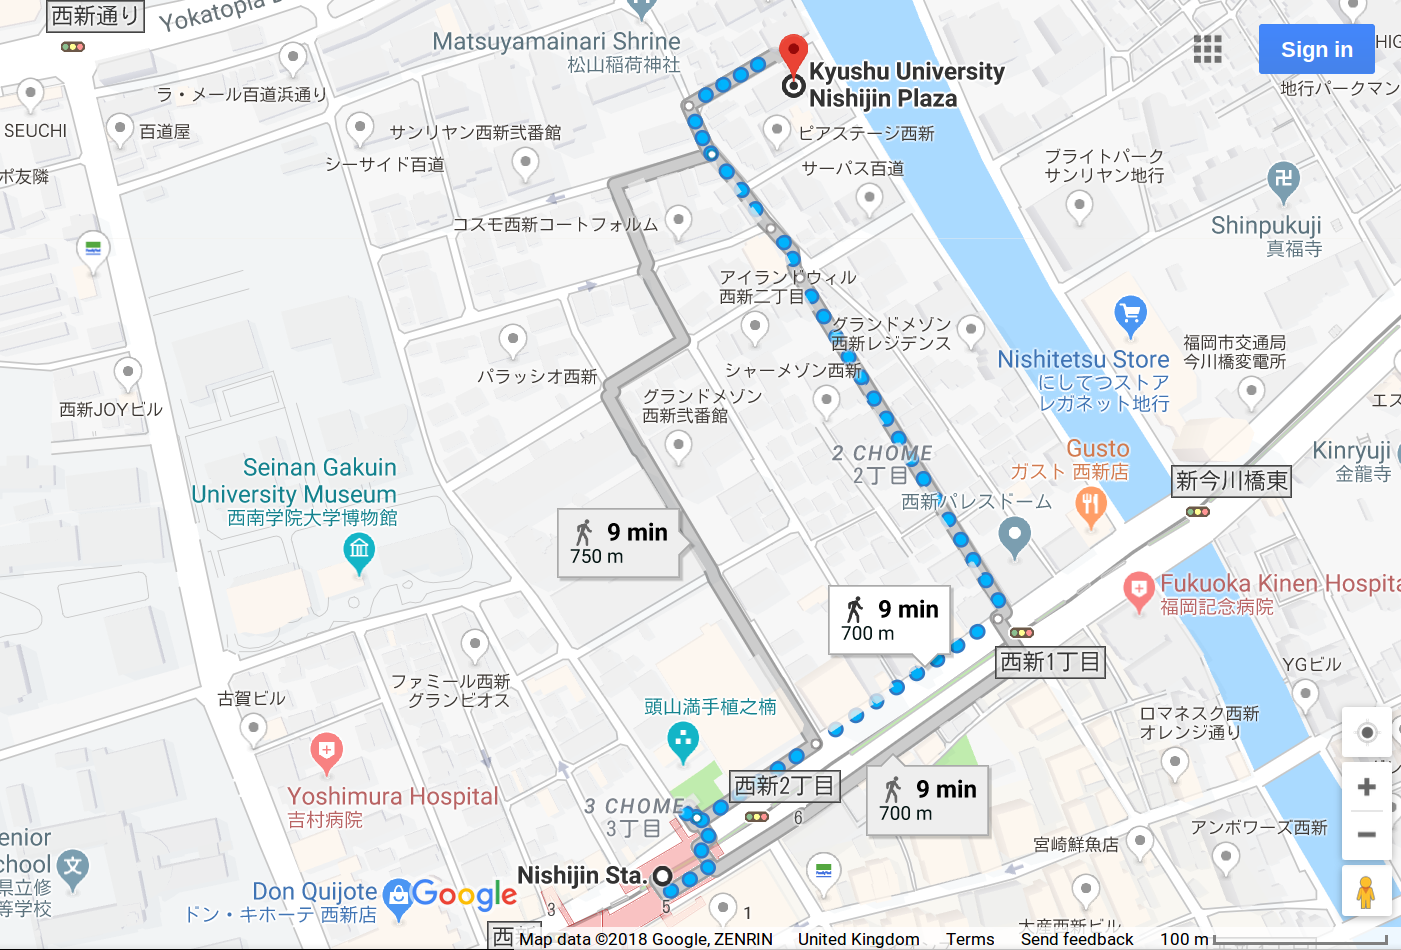
\includegraphics[width=\textwidth]{google_map01.png}


\includegraphics[width=0.25\textwidth]{google_map01_qr.png}

\newpage
\subsection*{Suginoya}
1442 Motooka, Nishi Ward, Fukuoka, Fukuoka Prefecture 819-0385, Japan

\noindent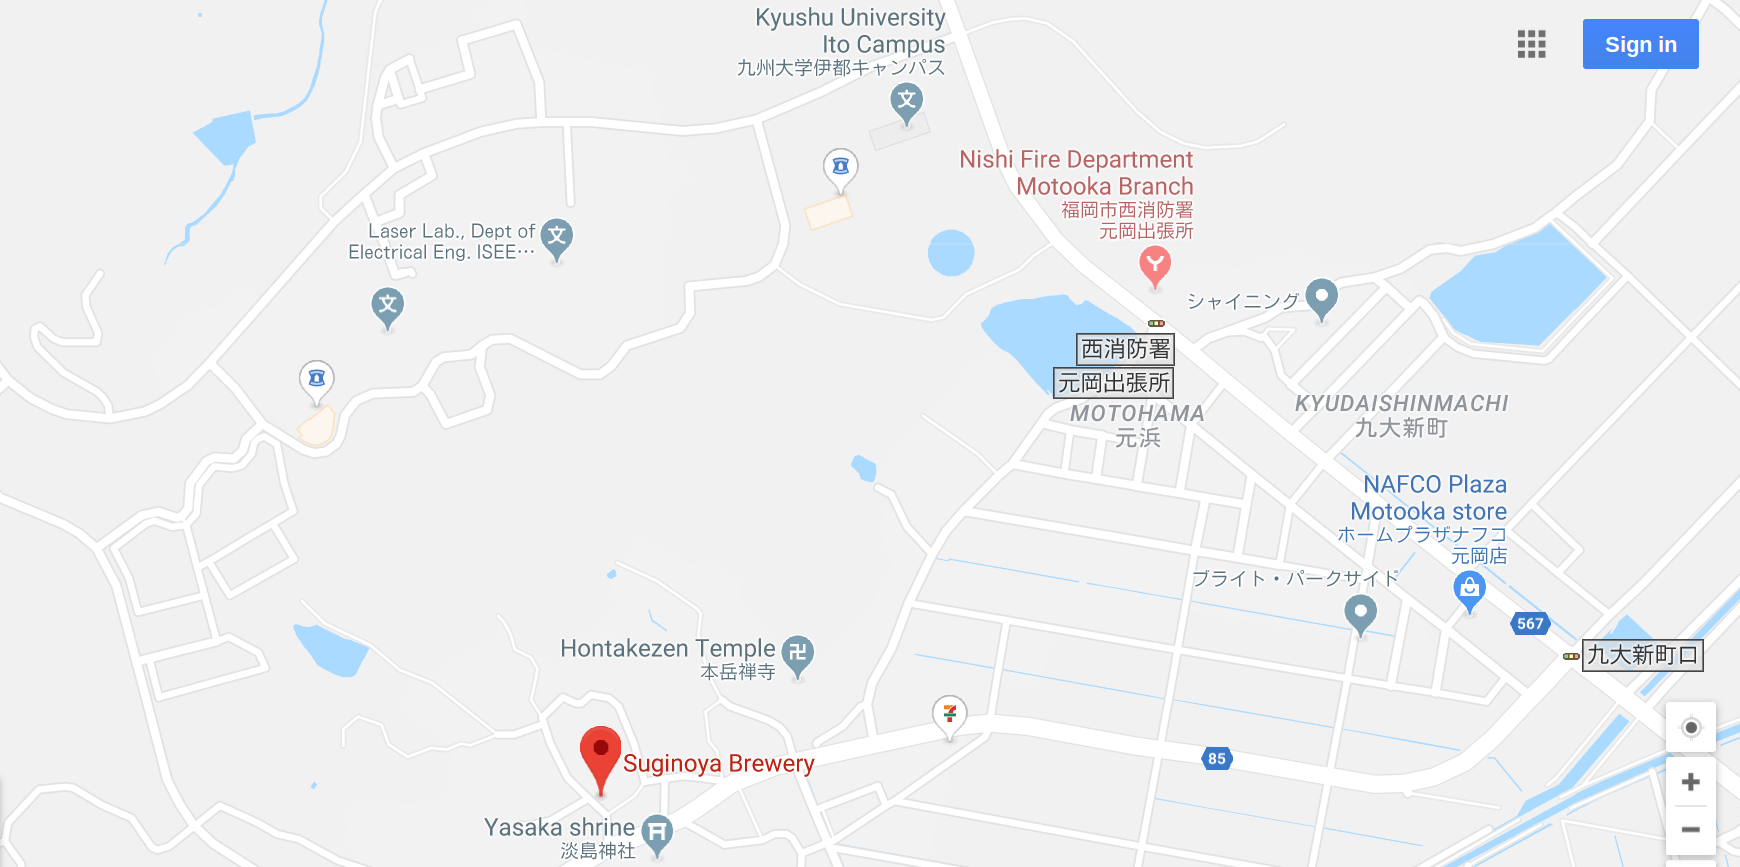
\includegraphics[width=\textwidth]{suginoya.png}

\newpage
\subsection*{Uminomichi}
B1,Tenjin Kimuraya Bldg, 1-12-3, Tenjin, Chuo-ku, Fukuoka-shi, Fukuoka-ken, 810-0001

\noindent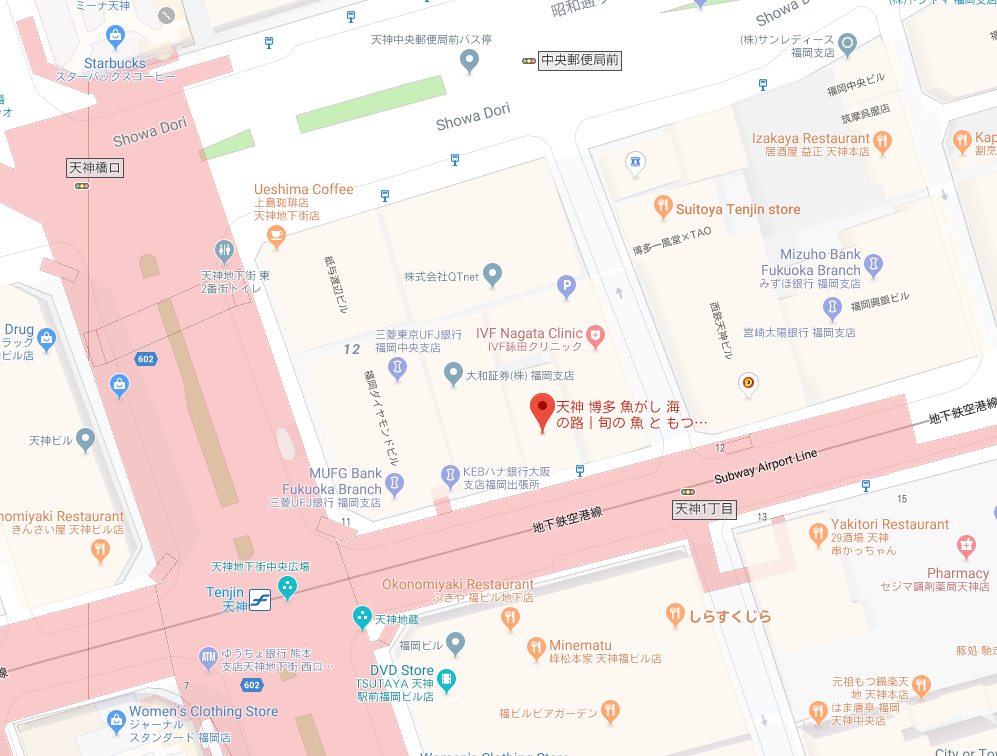
\includegraphics[width=\textwidth]{uminomichi.png}


\includegraphics[width=0.25\textwidth]{uminomichi_qr.png}

\newpage
\subsection*{Tour departure location}

Please arrive at the tour departure location in advance of the scheduled departure time, so that the
coach can leave on time.   
The meeting place is in front of the Fukuoka branch of the Bank of Japan, just a few minutes walk from Tenjin station.

\noindent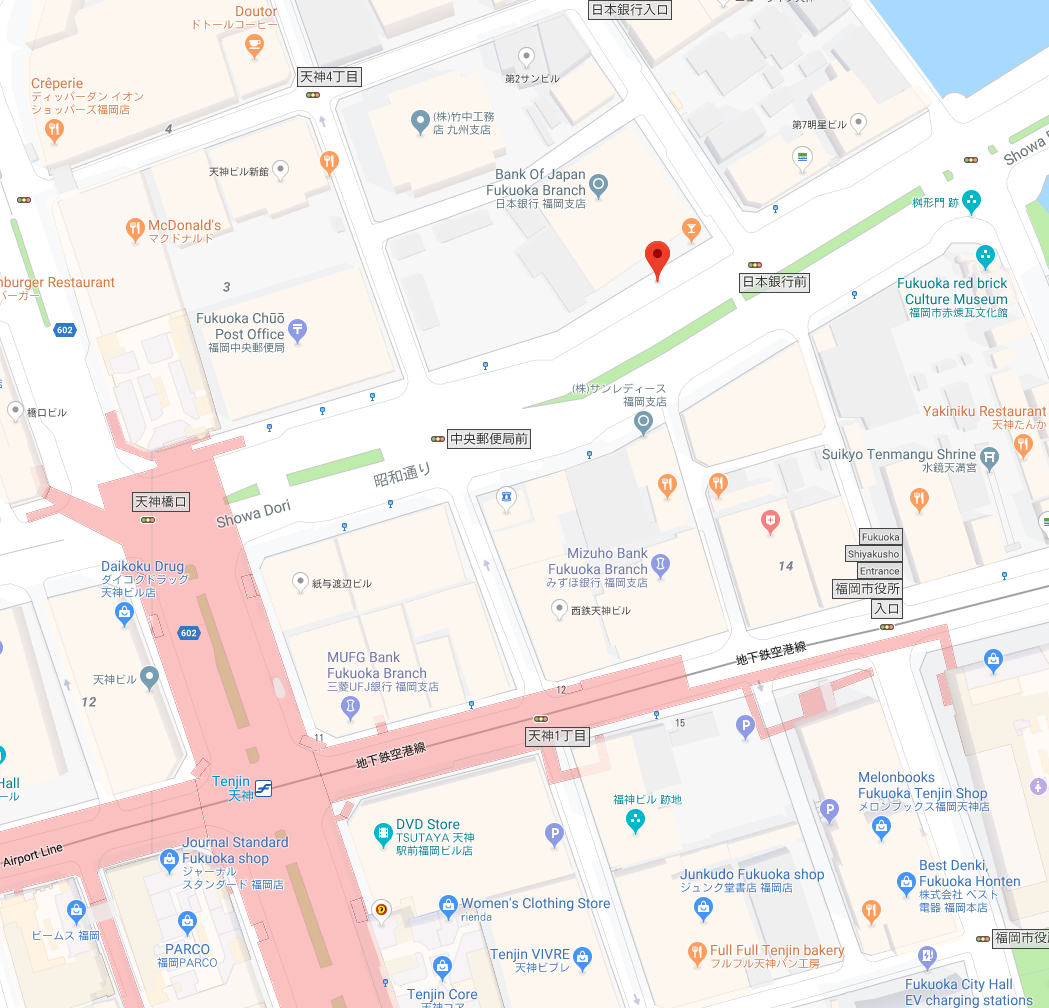
\includegraphics[width=\textwidth]{tour_meeting_place.png}

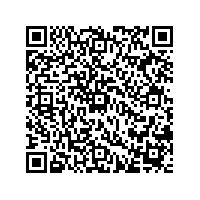
\includegraphics[width=0.25\textwidth]{tour_meeting_place_qrcode.png}


